\section{The Converged Optimizations Framework}
\label{sec:optimizations}

This section presents \name, a converged relational/graph optimization framework designed to optimize the query
processing of \spjm queries. We begin by introducing a naive solution built upon the graph-agnostic
method for solving the matching operator. We then delve into the converged workflow of \name, which leverages the graph-aware method for solving the matching operator and introduces a complete workflow that aims to integrate techniques from both relational and graph optimization modules.


%\begin{figure}
%    \centering
%    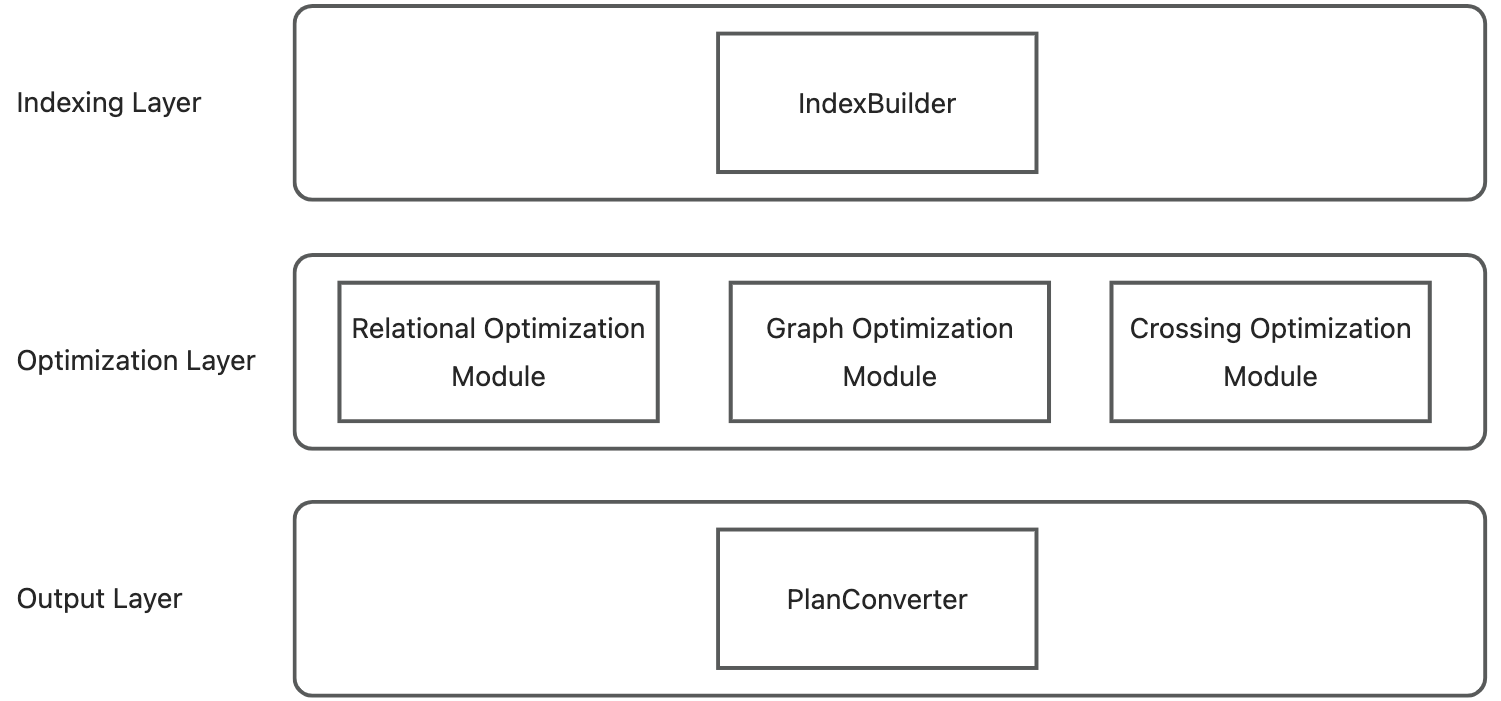
\includegraphics[width=\linewidth]{./figures/framework.png}
%    \caption{Overview of the Converged Graph Relational Optimization Framework.}
%    \label{fig:framework-overview}
%\end{figure}

\begin{figure*}
    \centering
    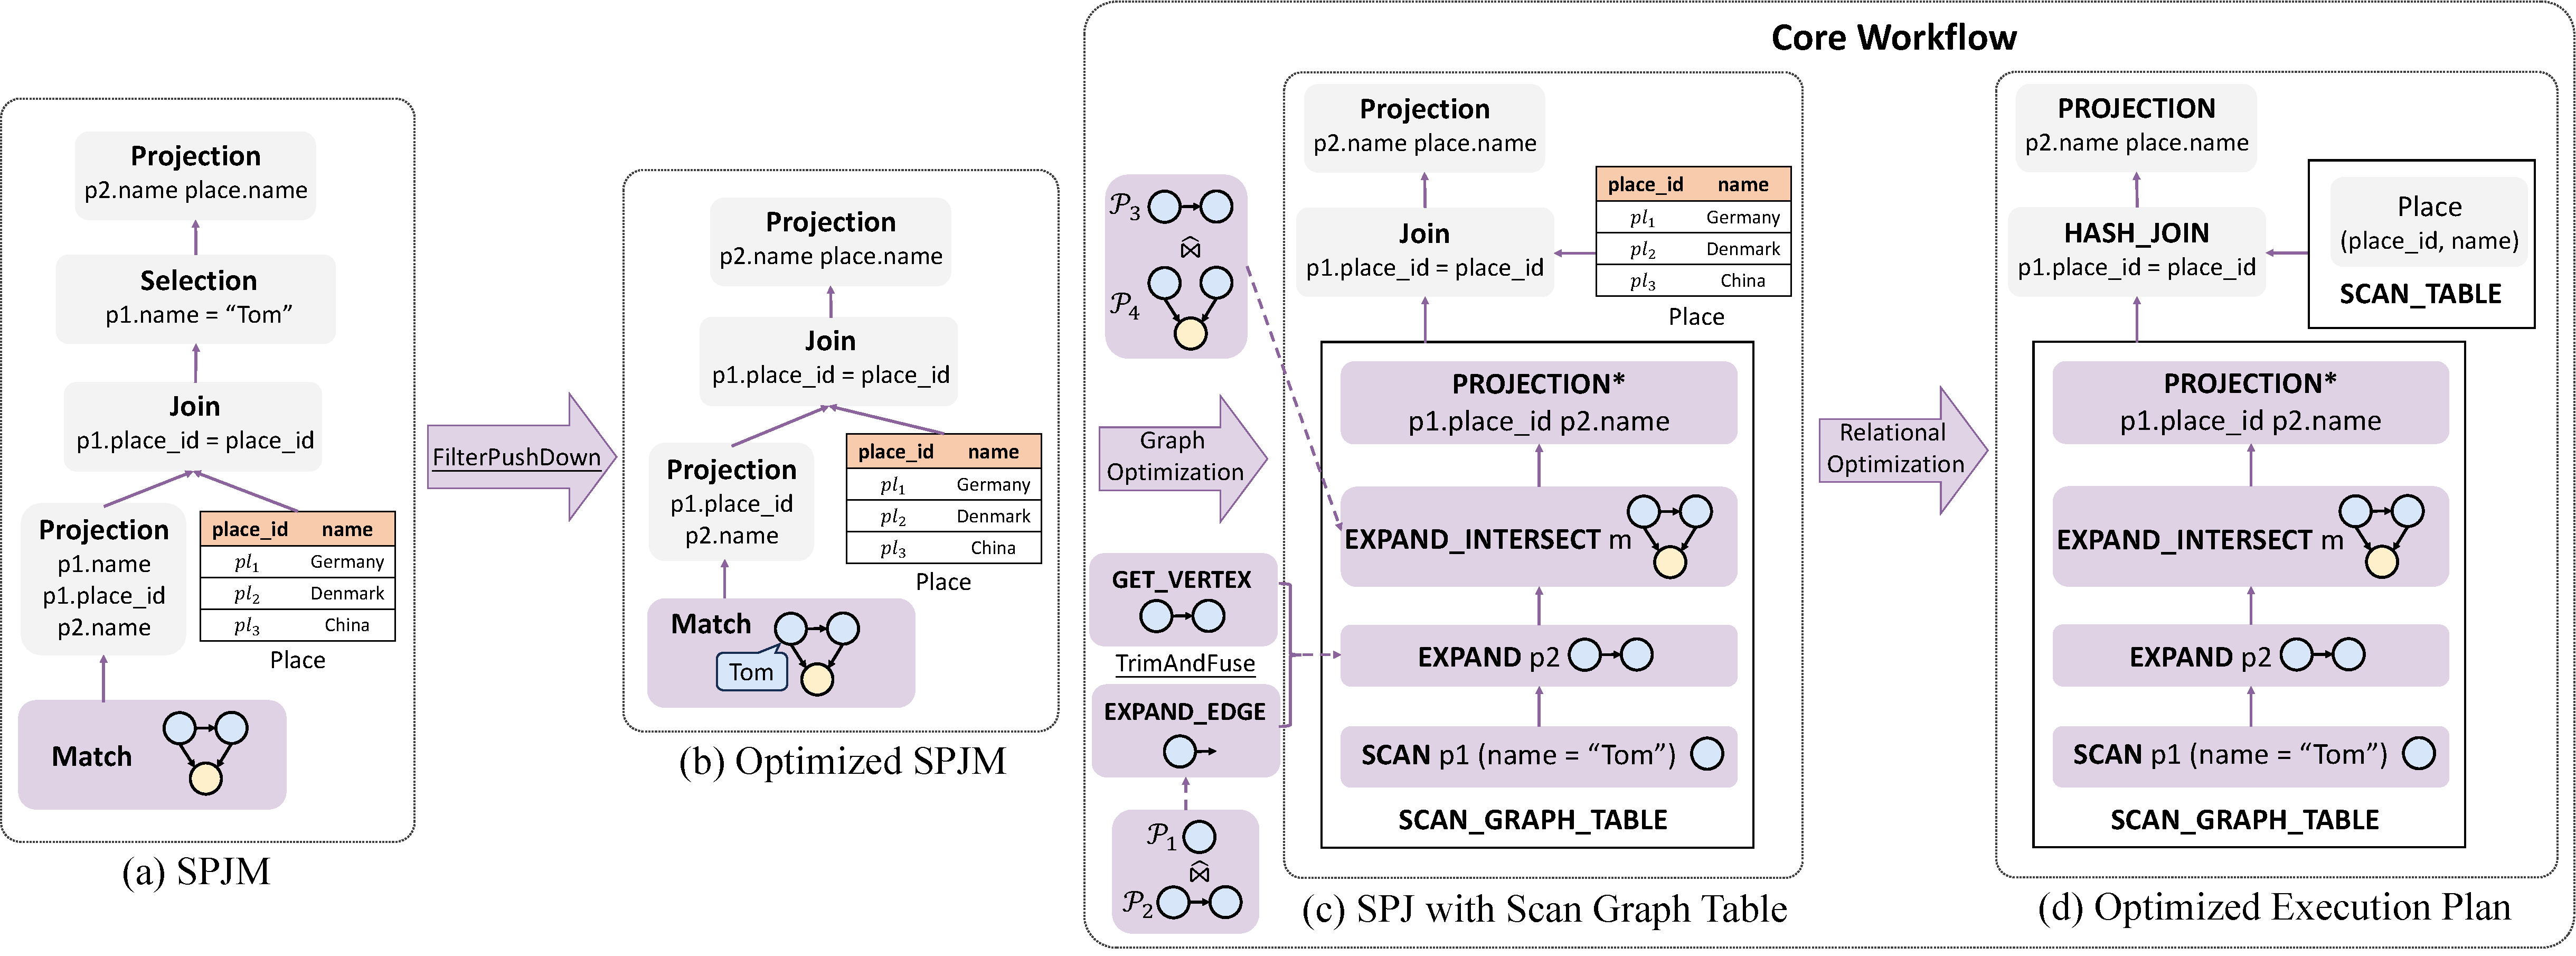
\includegraphics[width=\linewidth]{./figures/workflow.pdf}
    \caption{Converged Optimization Workflow}
    \label{fig:framework-workflow}
\end{figure*}


\subsection{Graph-Agnostic Optimizer}
\label{sec:relational-only}
The graph-agnostic optimizer is straightforward: it applies the graph-agnostic method to transform the matching operator in an \spjm query into a series of relational operations (\refeq{graph-agnostic}), effectively converting the \spjm query into an \spj query. The resulting \spj query can then be optimized by any existing relational optimizer, producing an execution plan. As an improvement, if a graph index (\refsec{graph-index}) is available, certain hash-join operators in the execution plan can be replaced by the predefined-join operator, as discussed in GrainDB~\cite{graindb}. The main advantage of this solution is its easy integration with any existing relational database. However, it suffers from two significant drawbacks that have been discussed in \refrem{graph-agnostic-vs-graph-aware}.

\subsection{The Converged Optimizer}
\label{sec:converged}
As illustrated in \reffig{framework-workflow}, the core workflow of the \name framework consists of two components: \emph{graph optimization} and \emph{relational optimization}. The graph optimization is responsible for handling the graph component in an \spjm query, leveraging graph optimization techniques to determine the optimal decomposition tree of the matching operator. On the other hand, the relational optimization takes over to optimize the relational component in the query.
The order in which these two components are applied is not strictly defined. However, for the purpose of our discussion, we will first focus on the graph optimization and then proceed to the relational optimization.
In addition to the core workflow, we further explore heuristic rules that highlight the non-trivial interplay between the relational and graph components in an \spjm query.

 %our analysis of real-life querying scenarios has revealed the need for a \emph{preposition optimizer}. This component is applied prior to the core workflow and is designed to apply heuristic rules.

%In addition to the primary component, we finally demonstrate the necessity of applying a \emph{preposition optimizer} component prior to the primary component.

\subsubsection{The Graph Optimization}
\label{sec:graph-optimizer}
In this work, we adopt the graph optimization techniques developed in \glogs~\cite{GLogS}. However, it is crucial to note that \glogs~ was originally designed for native graph data, whereas our framework deals with relational data, which necessitates a careful adaptation of \glogs's techniques to the relational setting.

\stitle{\glogue~Construction.} \glogs is built upon a data structure called \glogue, which is essentially a graph $\searchgraph_{\pattern}(V, E)$. In this graph, each vertex represents a pattern $\pattern'$ consisting of up to $k$ vertices (typically, $k=3$) that has non-empty matched instances in the original graph. There is an edge from $\pattern''$ to $\pattern'$, if there is a decomposition tree where $\pattern''$ is a child node of $\pattern'$.

 Each vertex $\pattern'$ in the \glogue maintains $|\matching(\pattern')|$, denoting the cardinality of the pattern. To reduce computation costs, \glogs employs a sparsification technique that constructs a smaller subgraph $G'$. The cardinality of the pattern can then be estimated using $|\matching_{G'}(\pattern')|$, computed based on the subgraph $G'$. In our work, we adapt this sparsification technique to construct the \glogue. To do so, we sample a subset of vertex and edge relations during the \rgmapping process. Once the subset of relations is obtained, they can serve as the input tables to the techniques presented in~\cite{gart} for constructing the sparsified graph $G'$.

\stitle{Cost Calculation.} The optimization process is essentially searching for the execution plan that incurs the minimal cost. Let the cost of an execution plan $\Phi$ for computing $\matching(\pattern)$ be $\cost_\Phi(\pattern)$. %The graph optimizer aims to find an optimal execution plan such that $\cost_\Phi(\pattern)$ is minimized. Clearly, this can be solved using dynamic programming~\cite{GLogS}.

Consider $\matching(\pattern') = \matching(\pattern'_l) \gjoin \matching(\pattern'_r)$ as an intermediate computation in an execution plan. We have:
\[
\cost_{\Phi}(\pattern') = \cost_{\Phi_l}(\pattern'_l) + \cost_{\Phi_r}(\pattern'_r) + \cost(\gjoin),
\]
where $\Phi_l$ and $\Phi_r$ are the execution plans for computing $\matching(\pattern'_l)$ and $\matching(\pattern'_r)$, respectively, and $\cost(\gjoin)$ is the cost of the join operation.

When a graph index is available, there are three physical implementations of $\gjoin$, depending on the type of $\pattern'_r$, and the calculation of $\cost(\gjoin)$ differs accordingly:
\begin{itemize}
\item If $\pattern'_r$ is a single-edge pattern, $\gjoin$ is implemented using \expandedge~ followed by \getvertex. The cost is calculated based on the cardinality of $\matching(\pattern'_l)$ (can be looked up in the \glogue) and the average degree of the graph, namely $|\matching(\pattern'_l)| \times \overline{d}$.
\item If $\pattern'_r$ is a complete star, $\gjoin$ is implemented using the \expandintersect~ operator. The cost is calculated based on the cardinality of $\matching(\pattern'_l)$ and the average intersection size of the neighbors of the vertices being intersected, which is maintained on the corresponding edge from $P'$ to $\pattern'_l$ in \glogue.
\item  If $\pattern'_r$ is any arbitrary pattern, $\gjoin$ is implemented as a \hashjoin. The cost is calculated as the product of the cardinalities of the two relations being joined, i.e., $\cost(\gjoin) = |\matching(\pattern'_l)| \times |\matching(\pattern'_r)|$.
\end{itemize}

In the absence of a graph index, \hashjoin~ is used for the entire plan, where the cost is simply the product of the cardinalities of the two relations being joined.

\comment{
\begin{example}
    As shown in \reffig{framework-workflow}, since $\matching(\pattern_2)$ is a single-edge pattern, the join operator between $\matching(\pattern_1)$ and $\matching(\pattern_2)$ is implemented using \expandedge~followed by \getvertex.
    Besides, as $\matching(\pattern_4)$ is a complete star, the join operator bewteen $\matching(\pattern_3)$ and $\matching(\pattern_4)$ is implemented using the \expandintersect~operator.
\end{example}
}

\stitle{Plan Computation.} Searching for the optimal execution plan in \name remains the same as in \glogs. The optimal plan is obtained by searching for the shortest path in the \glogue from the single-vertex pattern to the queried pattern.  %The process is repeated until the $\pattern$ node is reached, at which point the optimal execution plan is obtained.
\reffig{framework-workflow}(c) demonstrates a physical plan for matching the given triangle pattern when a graph index is present. The plan reflects the example in~\refex{physical-implementation}, with one exception: the pair of \expandedge and \getvertex operators is fused into a single \expand operator, which will be discussed as a heuristic rule called \joinfuserule.


\subsubsection{The Relational Optimization}
Once the graph optimizer has computed the optimal execution plan for $\matching(\pattern)$, the next step is to integrate this plan with the remaining relational operators in the \spjm query. The relational optimization is responsible for optimizing these remaining operators, which are all relational operators. Any existing relational optimizer can be used for this purpose.

%It's important to note that before $\matching(\pattern)$ can be integrated with the remaining relational component of the query, a specialized projection operator $\gproject$ must be applied to the matched results to flatten the graph relation into a relation, making it compatible with the relational operators. To facilitate this integration, we introduce a new physical operator called \scangraphtable, as shown in \reffig{framework-workflow}(c), which encapsulates the $\gproject$ operator and the optimal execution plan for $\matching(\pattern)$.

To prevent the relational optimizer delve into the internal details of the graph pattern matching process, we introduce a new physical operator called \scangraphtable, as shown in \reffig{framework-workflow}(c), which encapsulates the $\gproject$ operator and the optimal execution plan for $\matching(\pattern)$.
The \scangraphtable~ operator acts as a bridge between the graph and relational components of the query. From the perspective of the relational optimizer, \scangraphtable~ behaves like a standard \scan operator, providing a relational interface to the matched results. %This abstraction allows the relational optimizer to treat \scangraphtable~ as a regular relational operator, without the need to delve into the internal details of the graph pattern matching process.

\subsubsection{Heuristic Optimization Rules}
In real-life use cases, heuristic rules may involve non-trivial interactions between the relational and graph components of an \spjm query. We explore two representative rules, \filterrule~ and \joinfuserule, which can be applied at different stages of the optimization process to improve query performance.

\stitle{\filterrule.} To elaborate the rule, we extend the definition of a pattern $(\pattern, \constraints)$, introducing constraints within $\constraints$. For example, constraints can specify predicate $d$ such as $\id(v_1) = p_1$ for a vertex $v_1$, or $e_1.date > \text{"2024-03-31"}$ for an edge $e_1$. With the constraints defined, any matching result of $\pattern$ must have the corresponding vertices and edges adhering to the predicates.

Often while writing queries, users may not specify constraints on the pattern but rather use the selection operator after the matching results have been projected into the relational relation, which can be described as:
\[
\sigma_{d'_{v_a}} (\widehat{\pi}_{v.a \rightarrow \text{v\_a}, \ldots} \matching(\pattern))
\]
The predicate $d'_{v_a}$ defines a predicate in terms of an attribute of the pattern vertex that is projected by $\widehat{\pi}$ from the matched results. The motivation example in \refex{introduction:sqlpgq} illustrates such a case, where the selection predicate \kk{g.p1\_name = ``Tom''} is applied to the pattern vertex $v_{p_1}$.
There is wasteful computation if the selection is applied after the costly pattern matching. A more efficient approach is to push the selection predicate down into the matching operator.
%An extra benefit of doing so is that the optimizer can leverage the constraints to recalculate the cost, potentially generating better execution plans.
The \filterrule is formally defined as:
\begin{equation*}
\sigma_{\constraints} (\widehat{\pi}_{v.a \rightarrow \text{v\_a}, \ldots} \matching(\pattern)) \\
\equiv \sigma_{\constraints'} (\widehat{\pi}_{v.a \rightarrow \text{v\_a}, \ldots} \matching((\pattern, \{d_v\}))),
\end{equation*}
where $\constraints' = \constraints \setminus \{d'_{v_a}\}$, and $\{d_v\}$ is the corresponding constraints that are appended to the pattern $\pattern$.

It is recommended to apply the \filterrule before graph optimization, as this allows the optimizer to leverage the pushed-down constraints to recalculate the cost, potentially generating more efficient execution plans. \reffig{framework-workflow}(b) showcases the effects of applying the \filterrule, where the selection predicate \kk{g.p1\_name = ``Tom''} is pushed down into the matching operator.

\stitle{\joinfuserule.}
The \joinfuserule~ aims to optimize the query plan by fusing \expandedge, which expands edges, and \getvertex, which retrieves the associated vertices, where these two operators are typically paired in the physical implementation of the matching operator. This rule aims to combine the two operators into a single \expand~ operator that retrieves the neighboring vertices directly, to enhance the plan's efficiency.
However, this fusion strategy is conditional and precedes a critical examine-and-trim step to verify the necessity of edge properties provided by \expandedge.
If subsequent relational operations do not require any edge properties output by \getvertex~ (e.g., no property projection or filtering), the edge properties can be trimmed.
In this case, the \expandedge~ can be fused with the \getvertex~ to form a single \expand~ operator, which can directly retrieve the neighboring vertices by looking up the VE-index of the source vertex when the graph indices are available.
%
% The \joinfuserule~ aims to optimize the query plan by fusing \expandedge, which expands edges, and \getvertex, which retrieves the associated vertices, into a single \expand, which retrieves the neighboring vertices directly, to enhance the plan's efficiency.
% However, the fusion logical is not universally applicable, but relies on a preceded exam-and-trim procedure to determine whether the properties of the output vertices and edges are essential.
% For example, if subsequent relational operations do not require any vertex properties output by \getvertex~ (e.g., no property projection or filtering), the vertex properties can be trimmed.
% In this case, the \expandedge~ can be fused with the \getvertex~ to form a single \expand~ operator, and this fusion helps to eliminate the unnecessary join operation between the edge table and the associated vertex table to find the neighboring vertices, since the associated vertex ids (and labels) are already available in the adjacent edge table.
% Similarly, if the edge properties output by \expandedge~ are not required, it further optimize the fused \expand~ operation (with no edge properties required) by retrieving the neighboring vertices directly when the graph indices are available, which further eliminates the unnecessary join operation with the adjacent edge table.

\subsection{System Implementation}
We engineered the frontend of \name in Java and built it upon Apache Calcite~\cite{calcite}, a widely used open-source framework for data management, to utilize its robust relational query optimization infrastructure.
%The frontend of \name is responsible for parsing the input \spjm query, constructing the logical plan, and invoking the graph and relational optimizers to generate the optimal physical plan.
Firstly, we enhanced Calcite's SQL parser to recognize SQL/PGQ extensions, specifically to parse the \lstinline{GRAPH_TABLE} clause.
We created a new \lstinline{ScanGraphTableRelNode} that inherits from Calcite's core \lstinline{RelNode} class, translating the \lstinline{GRAPH_TABLE} clause into this newly defined operator within the logical plan.
Following the formation of the logical plan, the frontend invokes the converged optimizer to generate the optimal physical plan.
For the relational-graph interplay optimizations, we incorporate heuristic rules such as \filterrule and \joinfuserule into Calcite's rule-based HepPlanner, by specifying the activation conditions and consequent transformations of each rule.
For more nuanced optimization, we rely on the VolcanoPlanner, the cost-based planner in Calcite, to optimize the \lstinline{ScanGraphTableRelNode}.
We devised a top-down search algorithm that assesses the most efficient physical plan based on a cost model outlined in \refsec{graph-optimizer}, combined with high-order statistics from \glogue for more accurate cost estimation.
For the remaining relational operators in the query, we leverage Calcite's built-in optimizer, which already includes comprehensive relational optimization techniques.
Lastly, the converged optimizer outputs an optimized and platform-independent plan formatted with Google Protocol Buffers (protobuf) \cite{protobuf}. This ensures the adaptability of the \name framework's output to a variety of backend database systems.

We have developed the backend of the \name framework using C++, on top of DuckDB as the underlying relational execution engine, to demonstrate the optimization capabilities that \name can bring.
We integrated graph index support in GrainDB~\cite{graindb}. %, by building graph indices for predefined joins, as well as optimized sip join and merge sip join implementations (\todo{what is this}), leveraging the graph indices to speed up the execution, following the designs used in GrainDB~\cite{graindb}.
%Note we choose DuckDB instead of GrainDB directly as the backend, because DuckDB is more mature and incorporates advanced optimization techniques that are not yet available in GrainDB.
%However, we did bring in optimization features similar to those found in GrainDB to ensure that \name can take full advantage of the graph indices.
With graph index, the \expand, \expandedge~ and \getvertex~ operators can be optimized by directly using the predefined join in GrainDB.
Note that we craft a new implementation called merge sip join for the support of \expandintersect.
Without graph index, the \hashjoin~ operator is used throughout the entire plan.
To execute the optimized plans within DuckDB, we introduced a runtime module that translates the optimized physical plan into a sequence of DuckDB/GrainDB-compatible executable operators.
%For instance, the \expand~ operator is materialized using the merge sip join implementation, which significantly benefits from graph indices for processing efficiency.
%Moreover, for the \intersect~ operator, we crafted a new worst-case-optimal join implementation, which achieves better performance compared to the traditional multiple join that is not worst-case optimal in DuckDB.
This runtime module essentially bridges the gap between the optimized plans produced by the \name framework and DuckDB's execution engine, thereby validating \name's practicality and its potential to improve the performance of \spjm queries on an established relational database system.

% The \name system consists of three main components: the Metadata Provider, the Converged Optimizer, and the Plan Converter.
% The Metadata Provider maintains the metadata of the database, such as the schema information, the graph index information, and the statistics of the data.
% Specifically, we incorporated \glogue as a high-order statistics provider, which precomputed the small patterns with size up to $k$ (usually $k=3$) together with their cardinalities, for a more accurate cost estimation of the matching operator.
%This pre-computation are based on the sampled subsets of vertex and edge relations from the database, which are further constructed into a sparsified graph.

\comment{
In the Converged Optimizer,
we incorporated both graph optimization techniques and relational optimization techniques, to optimize the \spjm queries in a converged manner.
We use the rule-based optimization planner named HepPlanner in Calcite, to plug in heuristic optimization rules like \filterrule and \joinfuserule. We set up each rule by specifying the conditions under which it activates and the actions it takes once those conditions are met.
For more nuanced optimization, we employ the VolcanoPlanner, a cost-based optimization planner provided by Calcite, to optimize the match operator in a cost-based manner.
We have crafted a top-down search algorithm that calculates the most efficient physical plan for the match operator, leveraging the cost model outlined in \refsec{graph-optimizer}. The algorithm is informed by advanced statistics obtained from the Metadata Provider, ensuring a more precise cost estimation.
For the relational part, Calcite's built-in optimizer, which already includes comprehensive relational optimization techniques, is leveraged to fine-tune the rest of the relational operators in the query.
The Converged Optimizer generates its output as a unified plan formatted with Google Protocol Buffers (protobuf)\cite{protobuf}. This serialization format is both platform-independent and highly interoperable, facilitating the easy conversion of the unified plan into executable query plans tailored for the destination database system.
}
%To showcase the capabilities of the \name framework, we devised a Plan Converter that employs code generation techniques. This Plan Converter is adept at transforming the unified plan, produced by the Converged Optimizer, into executable code compatible with GrainDB, a relational database system that incorporates support for graph indices. This step is crucial in demonstrating the practical applicability and effectiveness of the \name framework in optimizing \spjm queries on a real-world relational database system.

\comment{
To optimize SPJM queries, we propose the converged graph relational optimization framework named relgo.
Specifically, optimizing SPJM queries with relgo is divided into three stages, i.e., preprocessing, optimizing, and converting.
In this section, we introduce the three stages of relgo in detail.

\subsection{Preprocessing Stage}
Given an SPJM query, relgo first parse the query and obtained the corresponding AST (Abstract Syntax Tree).
Then, the initial logical plan is obtained based on the AST.
Each node in the logical plan represents an operator, including the selection, projection, join, and scan operators.

Please note that the matching operator does not appear in logical plans, because it can be further decomposed into other operators such as join and selection operators.
Besides, according to \refdef{matching}, the output of the matching operator is a graph relation, and it is always followed by a projection operator $\widehat{\pi}$.
The output of $\widehat{\pi}$ is a relation and the matching operator as well as $\widehat{\pi}$ are considered as a whole as an implementation of the scan operator (named ScanMatchTable).

In the preprocessing stage, some universally effective optimizations can be applied to refine the plan in advance.
A typical optimization is \filterrule.

This rule is inspired by FilterPushdownRule in relational optimizer, which can push down the predicates to the scan operators to filter out invalid elements earlier.
Specifically, as the ScanMatchTable corresponding to $\matching(\pattern)$ is a physical implementation of the scan operator which acts like scanning a table obtained by matching $\pattern$, it is reasonable to integrate some filtering criteria into the ScanMatchTable operator.
Specifically, \filterrule finds predicates on the properties of elements in $\pattern$ and push them down into ScanMatchTable, so that invalid elements can be dropped earlier.
An example of applying \filterrule is given in Example \ref{example:push_down}.

Formally, the equation rule w.r.t.~\filterrule is as follows:
\begin{equation}
    \begin{split}
        & \pi_A(\sigma_{d}(R_1 \Join \cdots \Join R_m \Join \widetilde{R}) \\
        & \hspace*{2em} \equiv \pi_A(\sigma_{d_0}(R_1 \Join \cdots \Join R_m \Join \widetilde{R}_{d_1})), \\
        & \hspace*{4em} \text{where } \widetilde{R} = \widehat{\pi}_{attr*}(\mathcal{M}(\mathcal{P})) \\
        & \hspace*{4em} \text{and } \widetilde{R}_{d_1} = \widehat{\pi}_{attr*}(\mathcal{M}(\mathcal{P}_{d_1}))
    \end{split}
\end{equation}
where $d_1$ is a subset of $d$ with the constraints related to $\widetilde{R}$ and $d_0$ is obtained by removing $d_1$ from $d$.
Besides, $\mathcal{P}_{d_1}$ is obtained by adding constraints in $d_1$ to $\mathcal{P}$.

\subsection{Optimizing Stage}

Given a logical plan of a SPJM query, relgo optimizes the plan in the optimizing stage.
Specifically, the operations that appear in logical plans of SPJM queries often also appear in the logical plans of relational databases.
Therefore, typical relational optimizers, e.g., Calcite \cite{calcite}, can be employed to optimize this plan.

Besides, to optimize the implementation of ScanMatchTable, the matching plans are optimized with graph-aware methods.
Studies that optimize graph pattern matching can be utilized as the graph-aware methods, and when implementing \name, we leverage GLogS \cite{GLogS} to optimize matching plans.
Moreover, if graph indices are available, join operators in \expandvertex and \expandintersect can be implemented as predefined joins to further improve the efficiency.


\subsection{Converting Stage}

As different databases usually support different operators and their physical plans can be greatly varied, it is of critical importance for an optimization framework to be flexible.
Therefore, we implement a PlanConverter in the framework to ensure the flexibility.
Given the generated optimal physical plan, the PlanConverter transforms the plan to an internal representation (e.g., Substrait \cite{substrait}), and then the internal representation is transformed to the physical plan that can be executed by the target database.
Finally, the plan is executed and the query results are obtained.


The introduction of the framework is concluded with an example.


\begin{figure}
    \centering
    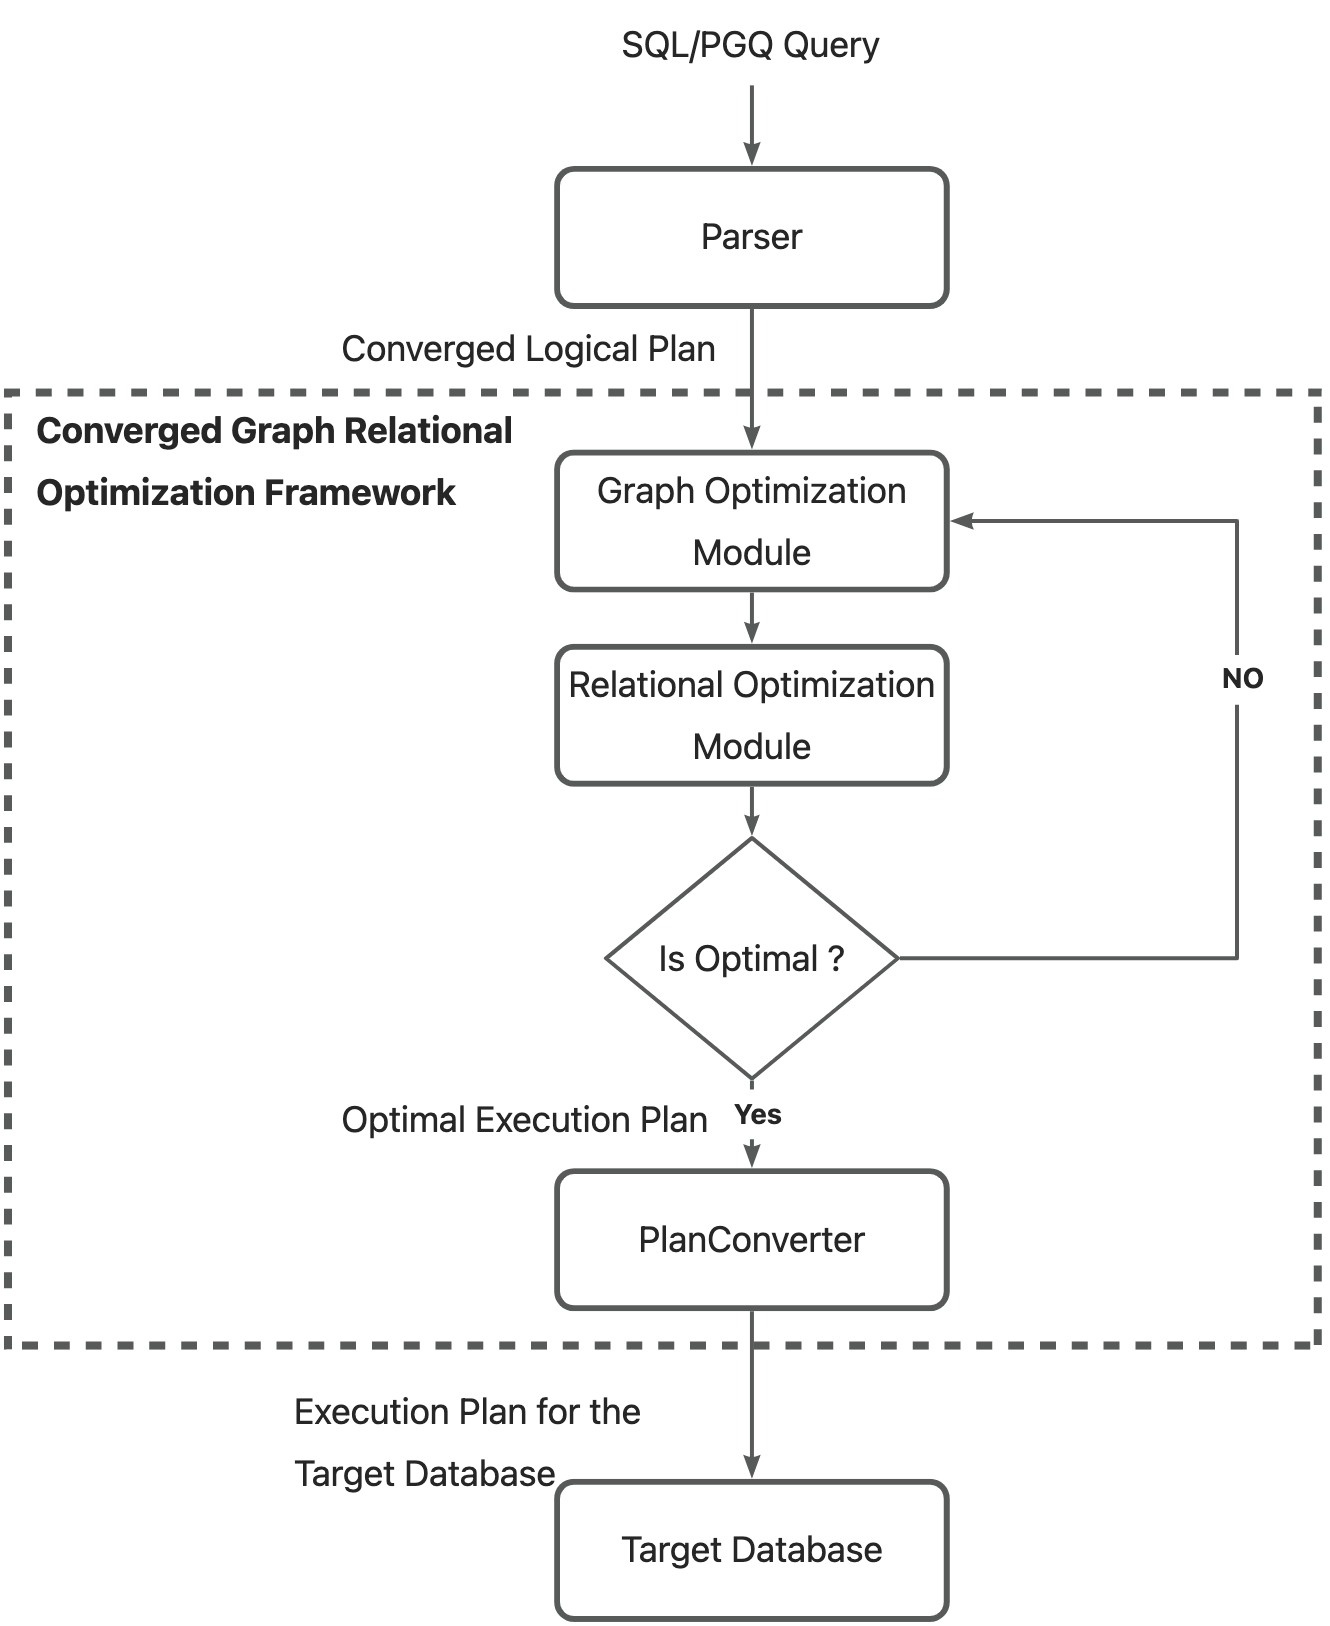
\includegraphics[width=.8\linewidth]{./figures/workflow.png}
    \caption{Workflow of the Converged Graph Relational Optimization Framework.}
    \label{fig:workflow}
\end{figure}

\begin{figure}
    \centering
    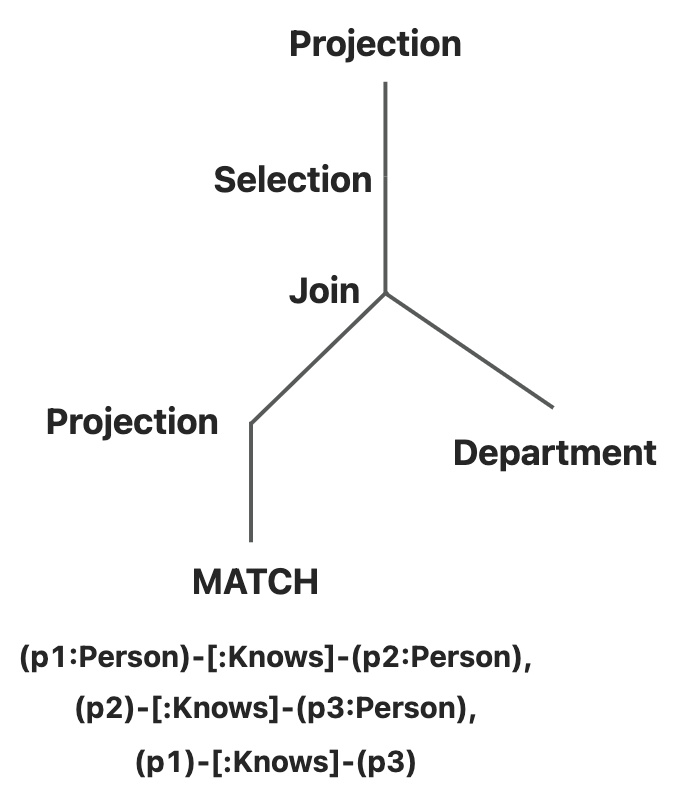
\includegraphics[width=.6\linewidth]{./figures/example_tree.png}
    \caption{The operator tree of SPJM query in Example \ref{example:framework}.}
    \label{fig:example-operator-tree}
\end{figure}

\begin{figure*}
    \centering
    \begin{subfigure}[b]{0.4\linewidth}
        \centering
        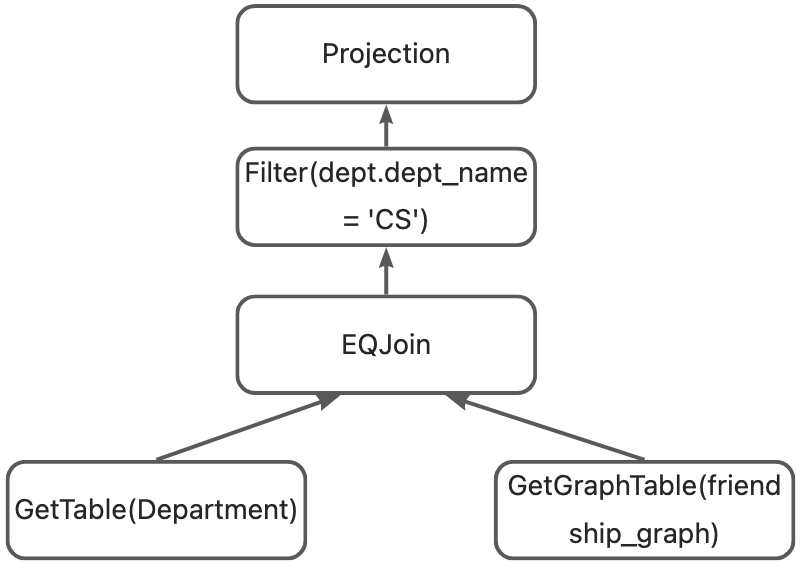
\includegraphics[width=\linewidth]{./figures/converged-logical-plan-relational.png}
        \caption{Outer query plan.}
        \label{fig:converged-logical-plan-relational}
    \end{subfigure}
    \begin{subfigure}[b]{0.4\linewidth}
        \centering
        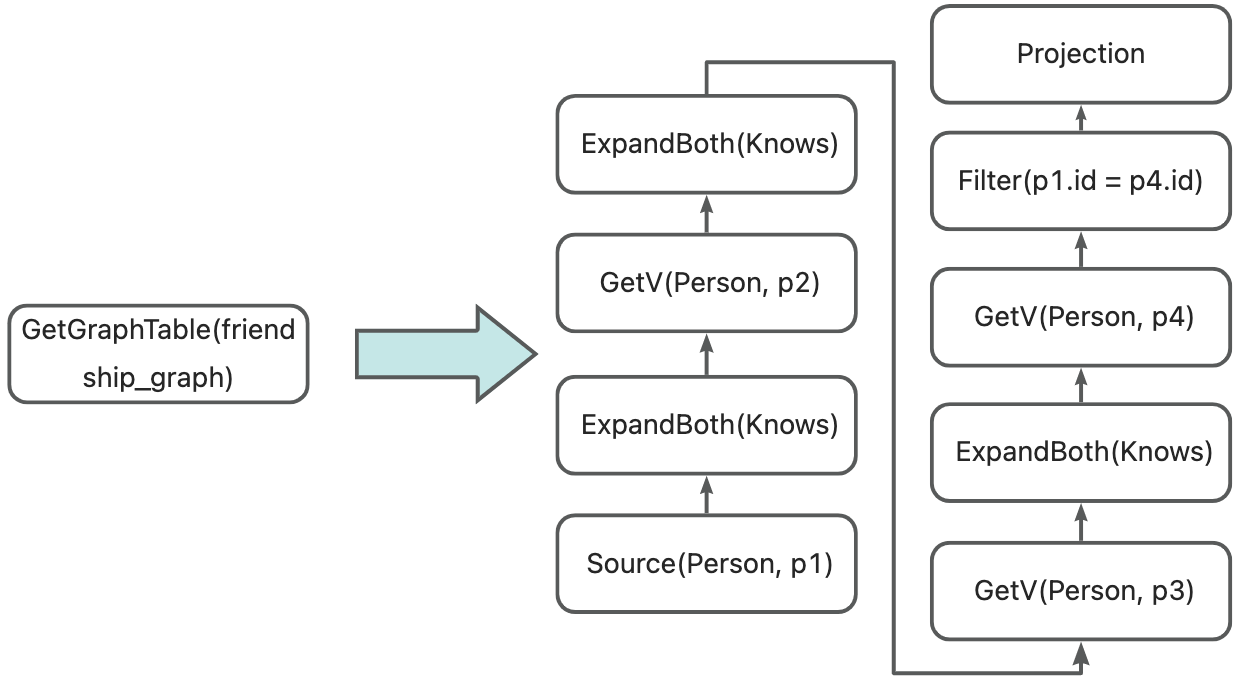
\includegraphics[width=\linewidth]{./figures/converged-logical-plan-graph.png}
        \caption{Match scanning plan.}
        \label{fig:converged-logical-plan-graph}
    \end{subfigure}
    \begin{subfigure}[b]{0.4\linewidth}
        \centering
        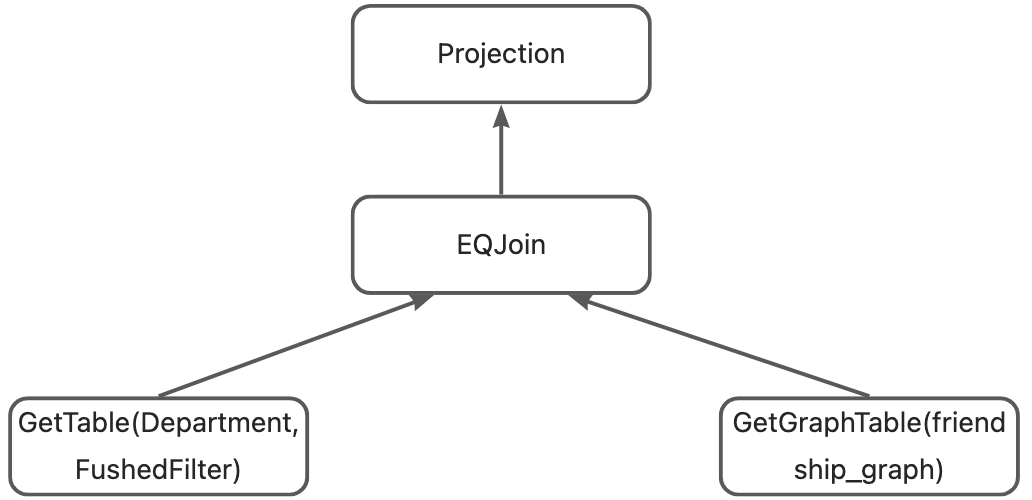
\includegraphics[width=\linewidth]{./figures/converged-logical-plan-relational-optimized.png}
        \caption{Outer query plan after Optimization.}
        \label{fig:relational-plan-optimized}
    \end{subfigure}
    \begin{subfigure}[b]{0.4\linewidth}
        \centering
        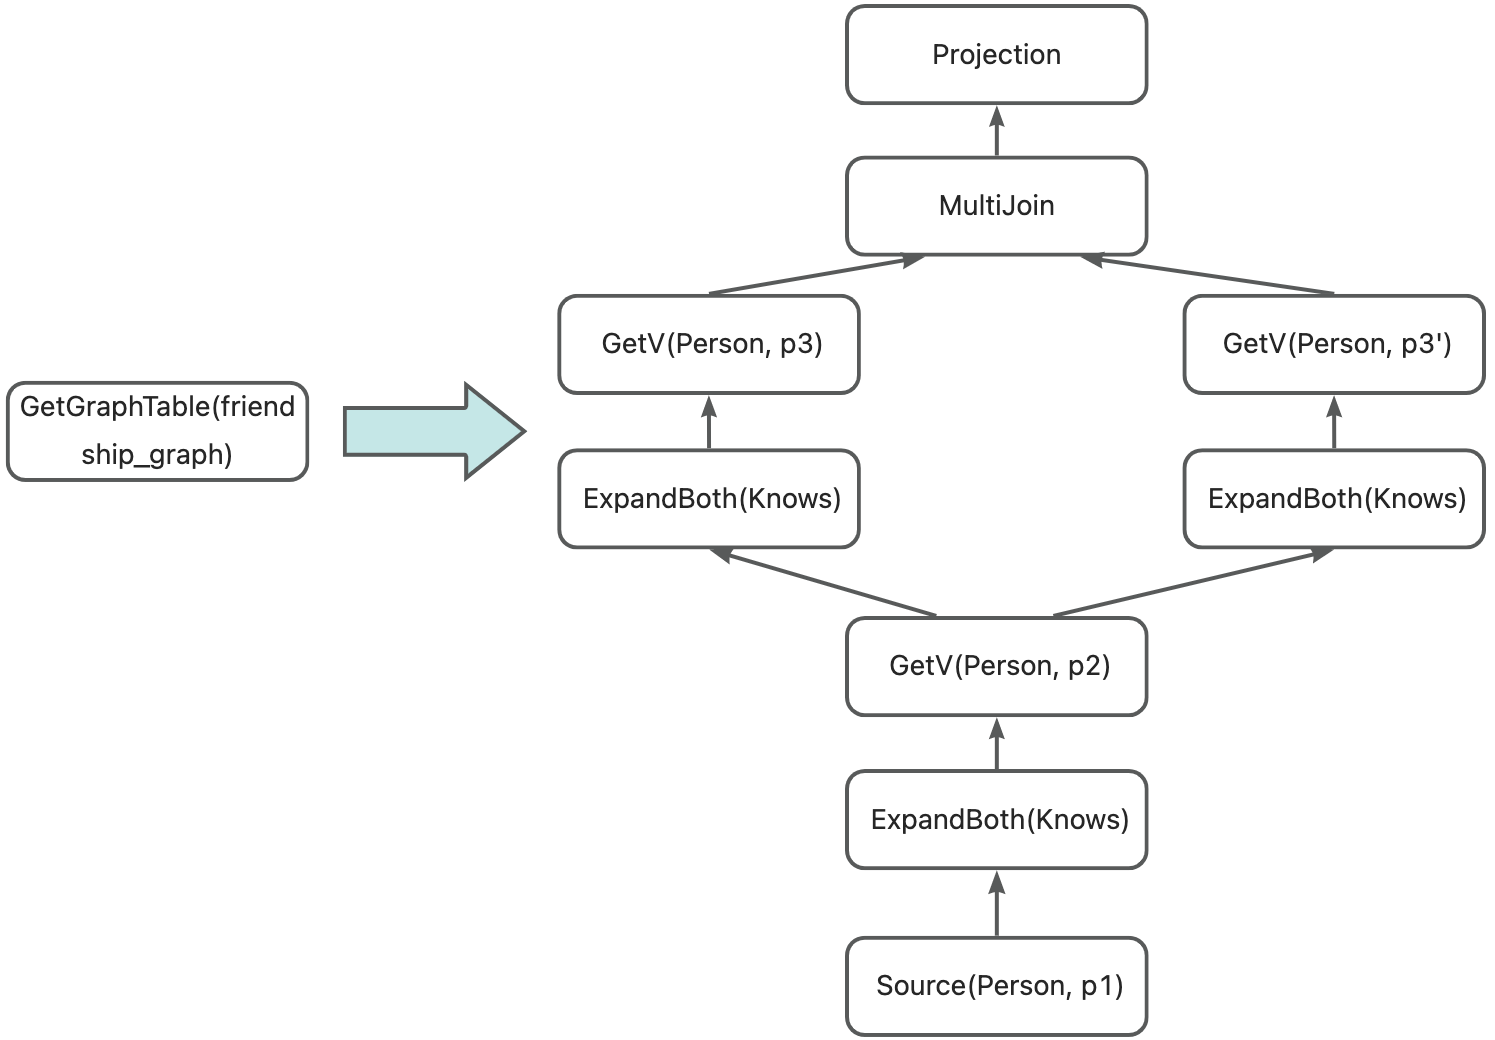
\includegraphics[width=\linewidth]{./figures/converged-logical-plan-graph-optimized.png}
        \caption{Match scanning plan after Optimization.}
        \label{fig:graph-plan-optimized}
    \end{subfigure}
    \begin{subfigure}[b]{0.5\linewidth}
        \centering
        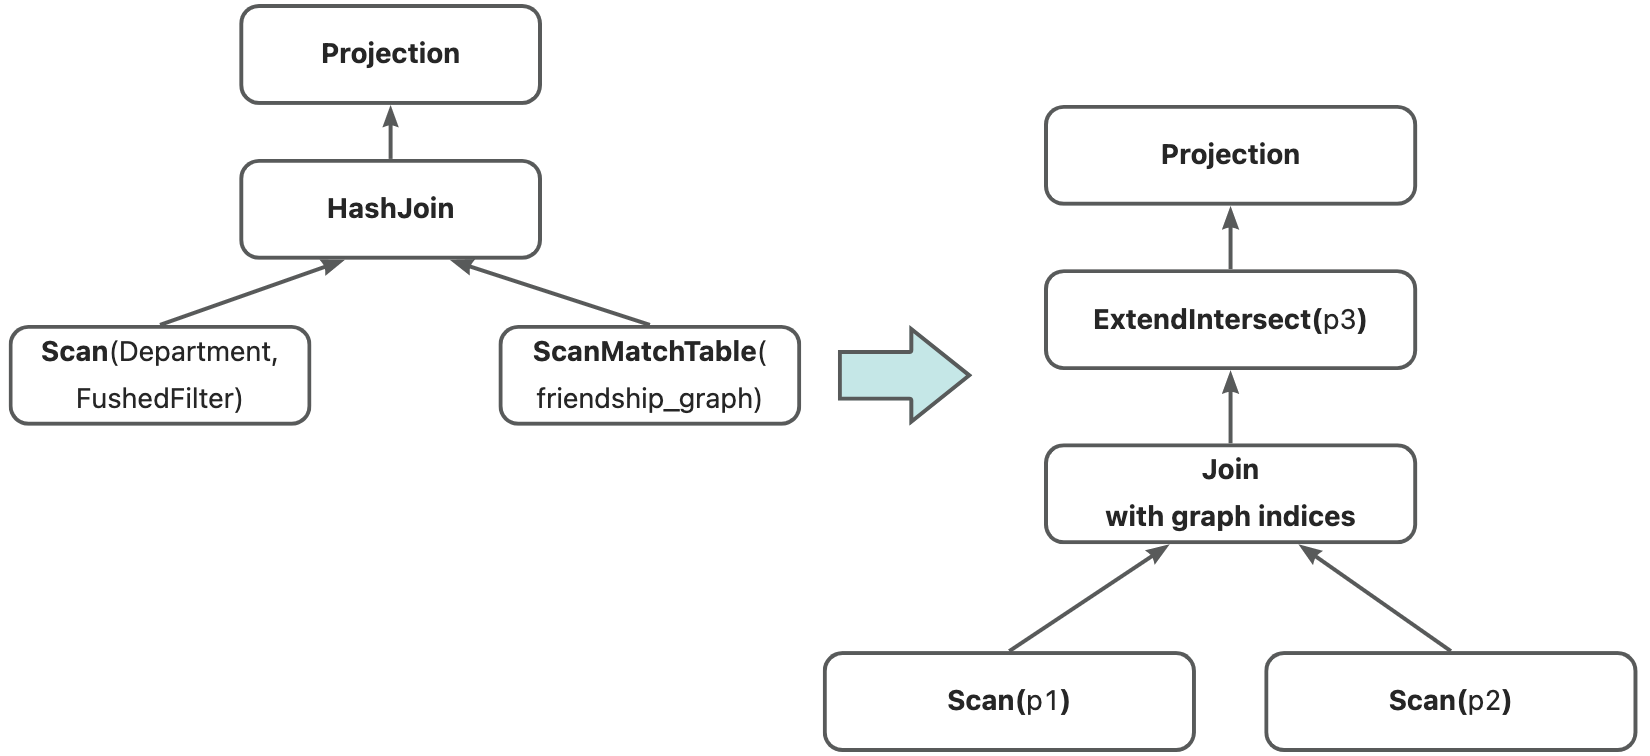
\includegraphics[width=\linewidth]{./figures/converged-physical-plan.png}
        \caption{Obtained Optimial Physical Plan.}
        \label{fig:physical-plan-optimized}
    \end{subfigure}
    \caption{An example of query opitmization.}
    \label{fig:query-grtree-example}
\end{figure*}



The above process of query processing is illustrated with the following example.

\begin{example}
    \label{example:framework}
    Given a relational database with tables as follows,
    \begin{equation*}
        \begin{split}
            & \textit{Person = (\underline{id}, name, dept\_id)} \\
            & \textit{Knows = (\underline{id1}, \underline{id2})} \\
            & \textit{Department = (\underline{dept\_id}, dept\_name)}, \\
        \end{split}
    \end{equation*}
    suppose we are going to find three persons satisfying:
    (1) These three persons know each other;
    (2) At least two of them are from the department of computer science.
    The SPJM query can be illustrated as shown in Fig.~\ref{fig:example-operator-tree}.

    In relational matching algebra, the SPJM query can be expressed as follows:
    Firstly, to obtain the triangles, the pattern $\mathcal{P}_{\triangle}$ is
    \begin{lstlisting}
        (p1:Person)-[:Knows]-(p2:Person),
        (p2)-[:Knows]-(p3:Person),
        (p1)-[:Knows]-(p3)
    \end{lstlisting}
    Then, to get the relational table that records the three person and their departments, the algebra expression is
    \begin{equation*}
        \begin{split}
            \widehat{R}_{graph} = & \pi_{p1.name\rightarrow pn1, p1.dept\_id \rightarrow dept1,p2.name\rightarrow pn2, p2.dept\_id \rightarrow dept2,} \\
            & _{p3.name\rightarrow pn3, p3.dept\_id \rightarrow dept3}(\mathcal{M}(GR, \mathcal{P}_{\triangle})),
        \end{split}
    \end{equation*}
    where $GR$ is a graph relation with only one tuple, and each attribute of the tuple is a vertex or an edge.
    The vertices correspond to rows in table Person and edges correspond to rows in table Knows.

    Finally, to obtain the triangles of persons with at least two persons from the department of computer science, the algebra expression is
    \begin{equation*}
        \begin{split}
        \pi_{pn1, pn2, pn3}
        (& \sigma_{dept.dept\_name = \text{`Computer Science'}}( \\
        & dept \Join_{dept1=dept.dept\_id \land dept2=dept.dept\_id} \widehat{R}_{graph})).
        \end{split}
    \end{equation*}

    Based on the above algebra expressions, the match scanning plan is shown in Fig.~\ref{fig:converged-logical-plan-graph} and the outer query plan is shown in Fig.~\ref{fig:converged-logical-plan-relational}.

    Then, optimization modules in the optimization layer are applied to optimize the plans.
    The optimized plans are shown in Fig.~\ref{fig:relational-plan-optimized} and Fig.~\ref{fig:graph-plan-optimized}.
    Moreover, the finally obtained optimal physical plan is shown in Fig.~\ref{fig:physical-plan-optimized}.
\end{example}
}
